%&pdflatex

\documentclass[12pt, letterpape]{article}
\usepackage{graphicx}
%\graphicspath{ }
 
\begin{document}

The universe is immense and it seems to be homogeneous, 
in a large scale, everywhere we look at.
 
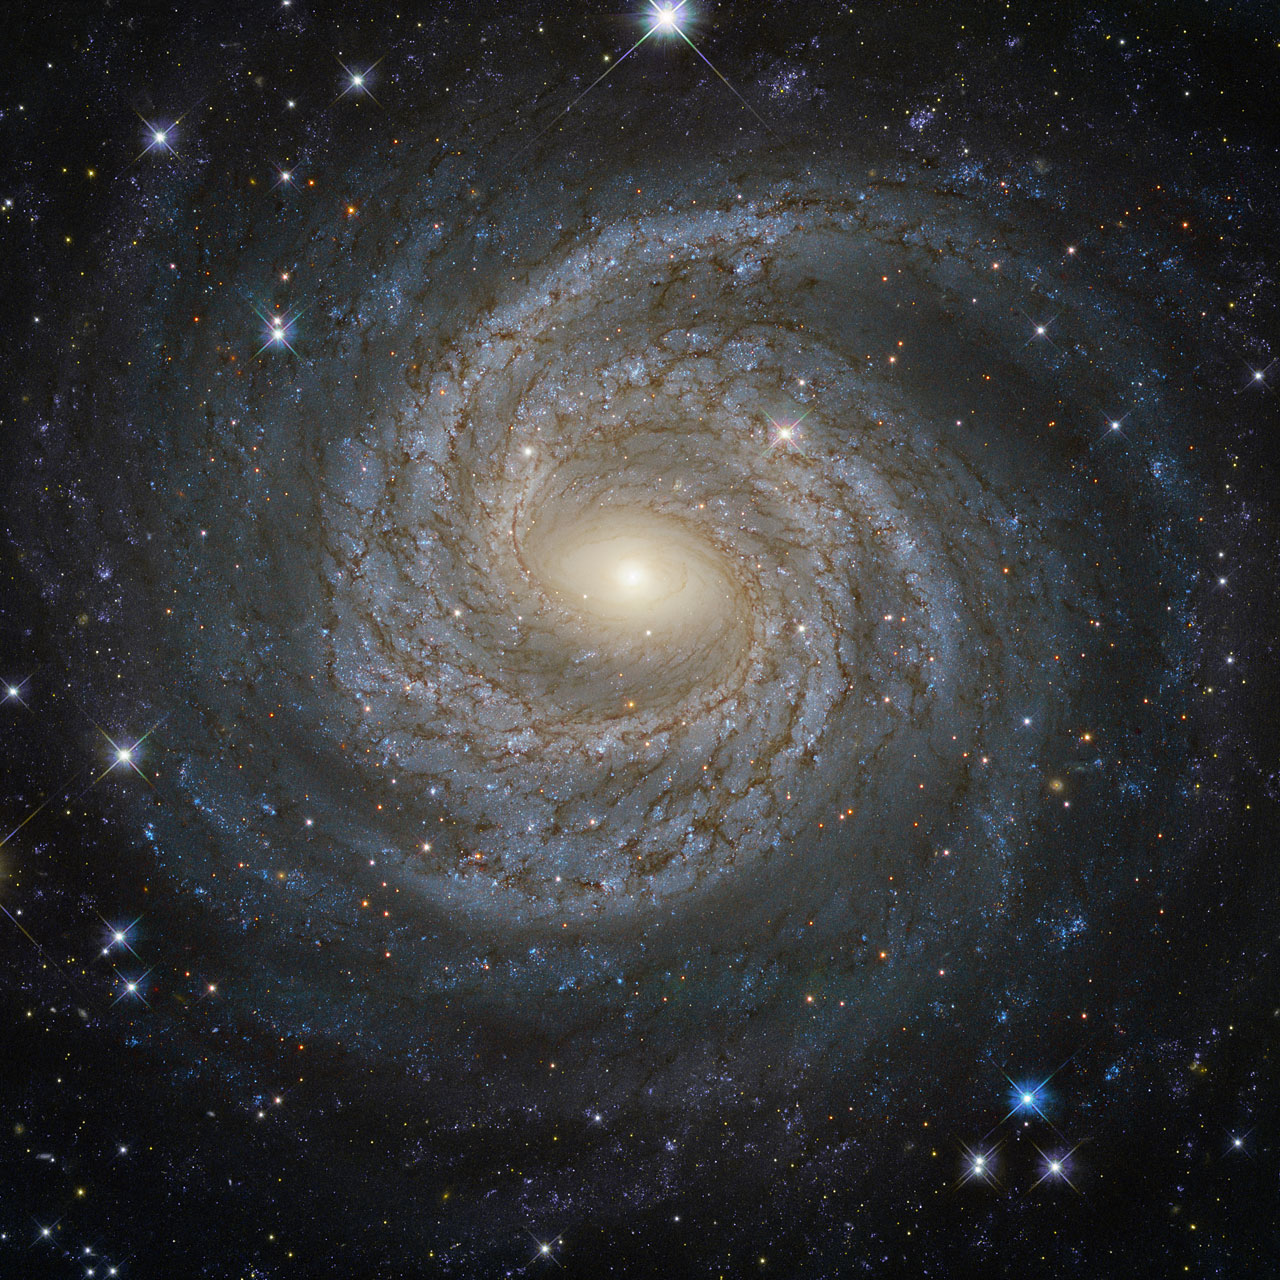
\includegraphics[scale=0.1]{image.jpg}
 
 {\fontfamily{bch}\selectfont
There's a picture of a galaxy above
}

\begin{figure}[h]
    \centering
    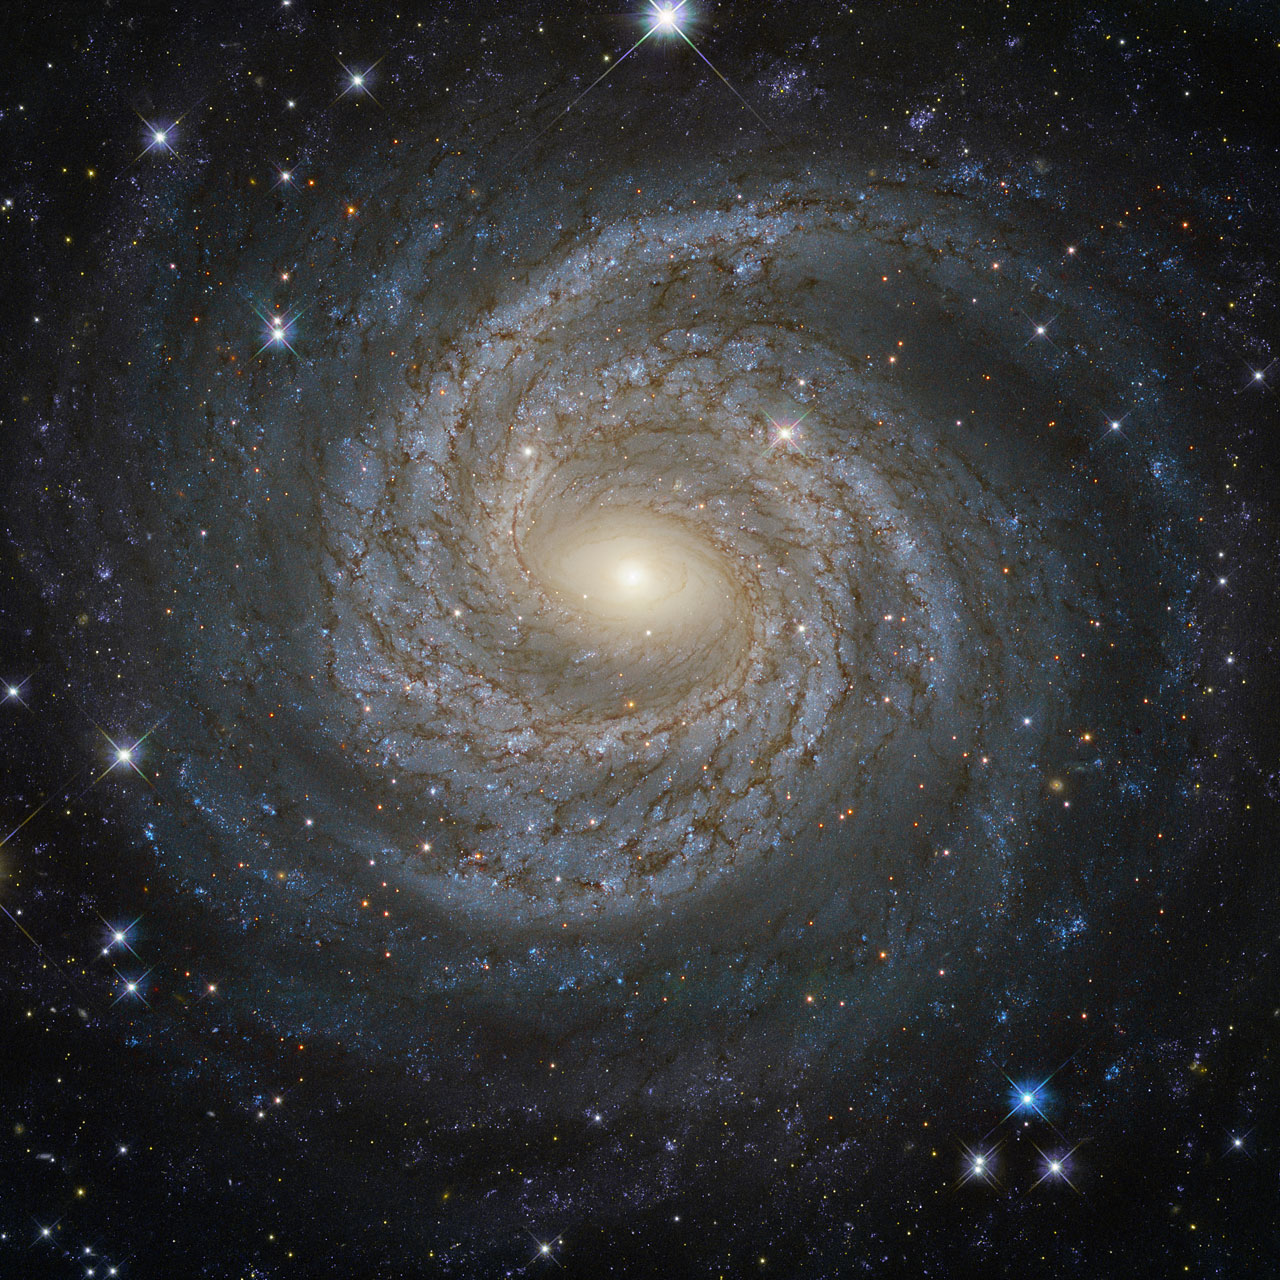
\includegraphics[width=0.25\textwidth]{image.jpg}
    \caption{a nice plot}
    \label{fig:mesh1}
\end{figure}

As you can see in the figure \ref{fig:mesh1}, the 
function grows near 0. Also, in the page \pageref{fig:mesh1} 
is the same example.

\begin{itemize}
  \item The individual entries are indicated with a black dot, a so-called bullet.
  \item The text in the entries may be of any length.
\end{itemize}


\end{document}